\documentclass{article}

\usepackage[dutch]{babel}
\usepackage[margin=3cm]{geometry}
\usepackage{graphicx}
\usepackage{float}
\usepackage{caption}
\usepackage{hyperref}
\usepackage{amsmath}
\usepackage{wrapfig}
\usepackage[parfill]{parskip}

% fonts
\usepackage[T1]{fontenc}
\usepackage{helvet}
\renewcommand{\familydefault}{\sfdefault}

\graphicspath{{img/}}

\newtheorem{theorem}{Definitie}[section]

\usepackage{enumitem}

\newenvironment{thmenum}
 {\begin{enumerate}[label=\upshape\bfseries(\roman*)]}
 {\end{enumerate}}

\usepackage{minted}
\setminted{frame=single,framesep=3pt,linenos}
\usepackage{upquote}
\usepackage{color}

\begin{document}

\begin{titlepage}
    \author{Tuur Vanhoutte}
    \title{Big Data}
\end{titlepage}

\pagenumbering{gobble}
\maketitle
\newpage
\tableofcontents
\newpage

\pagenumbering{arabic}

\section{Understanding Data Intensive Applications}

\subsection{Why Big Data?}

\subsubsection{Use case: data intensive application RouteYou}

\begin{figure}[H]
    \centering
    \includegraphics[width=0.5\textwidth]{routeyou.png}
    \caption{RouteYou}
\end{figure}

\begin{itemize}
    \item Routes - user preferences \& interests
    \item Searcheable Text data
    \item Geospatial data
    \item Community driven
    \begin{itemize}
        \item Exponential user growth is necessary to make the application posssible
        \item Server power/bills should grow linearly
    \end{itemize}
\end{itemize}

\subsection{Data Intensive Application: RAMS!}

\begin{itemize}
    \item \textbf{Reliable}
    \begin{itemize}
        \item tolerating human mistakes
    \end{itemize}
    \item \textbf{Available}
    \item \textbf{Maintainable}
    \begin{itemize}
        \item Easy to adapt (evolvability)
        \item Easy to deploy \& operate (operations/sys admins)
    \end{itemize}
    \item \textbf{Scalable}
    \begin{itemize}
        \item User growth while maintaining low response times
    \end{itemize}
\end{itemize}

\subsubsection{Common similar abbreviations}

\begin{itemize}
    \item Infrastructure: RAS (Reliable, Available, Serviceable)
    \item Developer: RMS (Reliable, Maintainable, Scalable)
\end{itemize}

\subsubsection{Methods to improve Maintainability}

\begin{itemize}
    \item Github
    \item Error handling
    \item Relative paths (not absolute)
    \item Abstraction (REST API, \dots)
    \item Documentation
\end{itemize}

\subsubsection{RAMS applied to RouteYou application}

\begin{itemize}
    \item Geospatial data (longitude, latitude)
    \item Available \& scalable
    \item Scalable \& low response time
    \item Community driven - unstructured text
    \item Maintainable: automatic classification of community input (ML)
\end{itemize}

\begin{figure}[H]
    \centering
    \includegraphics[width=0.5\textwidth]{RAMS-routeyou.png}
    \caption{To support many users, you need a caching layer}
\end{figure}


\subsection{Learning outcome for this module}

Being able to make infrastructure \& software choices to 
build a Reliable, Available, Maintainable \& Scalable (RAMS) 
data intensive application.

\begin{itemize}
    \item Deep insights into database technology \& cloud services
    \item Connecting with Machine Learning \& AI
    \item Configuring a data back-end (in the cloud or locally)
\end{itemize}


\subsection{Scaling}
\subsubsection{MySQL scaling}

\begin{figure}[H]
    \centering
    \includegraphics[width=0.5\textwidth]{mysql-scaling.png}
    \caption{Transactions/sec }
\end{figure}

\begin{itemize}
    \item Processing power of 16-64 = slightly less then 4x
    \item Real performance: 2.3x
    \item = scaling up: add more processing power to the system
\end{itemize}

\subsubsection{ElasticSearch Scaling: distributed system}

\begin{figure}[H]
    \centering
    \includegraphics[width=0.5\textwidth]{elasticsearch-scaling.png}
    \caption{Response time per request}
\end{figure}

\begin{itemize}
    \item Scaling out: add more servers to your data system
\end{itemize}

\subsubsection{Professional architecture (Dev oriented)}

\begin{figure}[H]
    \centering
    \includegraphics[width=0.5\textwidth]{professional-architecture.png}
    \caption{Professional architecture diagram}
\end{figure}


\begin{itemize}
    \item \textbf{Reverse proxy / Load balancer:} improves scalability
    \item \textbf{Opcode/app/Webserver:} webservice + API
    \item \textbf{Key-value store:} `caching layer'
    \item \textbf{Database server:} distributed storage system + relational database
\end{itemize}

\subsubsection{Time series Distributed database (OpenTSDB, InfluxDB)}

\begin{figure}[H]
    \centering
    \includegraphics[width=0.5\textwidth]{time-series-distributed-db.png}
    \caption{Data from windmill sensors. Most sensors log about every second}
\end{figure}

\begin{itemize}
    \item Losing data is not that big a problem
    \item Massive amount of data to write 
\end{itemize}

\subsection{Scalability \& application performance management}

Response times and percentiles rule the web

\subsubsection{The need for speed: some insights from Google}

\begin{itemize}
    \item Speed is a ranking factor
    \item When your site has high response times, less URLs will be crawled from your site
    \item 53\% of visits are abandoned if a site takes longer than 3 seconds to load
    \item Slow websites will be labeled by Google Chrome
\end{itemize}

\subsubsection{Response times for websites}

\begin{itemize}
    \item \textbf{Ideal:} "blink of an eye" is 300-400 ms
    \item \textbf{Excellent:} 500ms to 1.5 seconds at most
    \item \textbf{Barely acceptable:} 3 seconds
\end{itemize}

Response time = Network latency + processing

\begin{itemize}
    \item 2.9 seconds is faster than 50\% of the web
    \item 1.7 seconds is faster than 75\% of the web
    \item 0.8 seconds is faster than 94\% of the web
\end{itemize}

\subsubsection{4 components of network latency}

\begin{figure}[H]
    \centering
    \includegraphics[width=0.5\textwidth]{network-latency.png}
    \caption{Network latency diagram}
\end{figure}

\begin{itemize}
    \item Processing delay
    \begin{itemize}
        \item Processing network software stack (TCP/IP layers)
        \item Routing decisions
    \end{itemize}
    \item Transmission delay
    \begin{itemize}
        \item Bits on physical link (Bandwidth plays a big role, ex: 1Gbit/s)
    \end{itemize}
    \item Propagation delay
    \begin{itemize}
        \item Speed of EM signals in fiber: 200.000 km/s (67\% of lightspeed)
        \item Changes with distance and medium (Copper: 64\% of lightspeed)
    \end{itemize}
    \item Queing delay
    \begin{itemize}
        \item Time spent in router \& NIC buffers
    \end{itemize}
\end{itemize}

\subsubsection{TCP Congestion Window - slow start}

\begin{itemize}
    \item Network congestion = a network node or link is carrying more data than it can handle
    \item The internet is built around dropped packages
\end{itemize}

\begin{figure}[H]
    \centering
    \includegraphics[width=0.5\textwidth]{tcp-congestion-window.png}
    \caption{TCP Congestion window}
\end{figure}

\begin{itemize}
    \item 4-8-16-32 TCP segments (Win 2008, Win7)
    \item 10-20-40 (Linux 2.6+, Windows Server 2016 / Windows 10)
\end{itemize}

\begin{figure}[H]
    \centering
    \includegraphics[width=0.5\textwidth]{tcp-handshakes.png}
    \caption{Because of many handshakes, there is a lot of latency}
\end{figure}

\begin{itemize}
    \item Solution: KeepAlive of a HTTP Persistent Connection
    \begin{itemize}
        \item Only one 3-way handshake for many requests
        \item Lower network \& CPU load
        \item Lower response times
        \item \textbf{Downside}: more connections open $\Rightarrow$ more memory, more connection failures, app crashing, \dots
    \end{itemize}
\end{itemize}

\begin{itemize}
    \item Measure parallel requests of a website using \url{https://www.webpagetest.org/}
    \item Get a waterfall view of a webpage
\end{itemize}

\subsubsection{Long tail latency}

\begin{figure}[H]
    \centering
    \includegraphics[width=0.5\textwidth]{long-tail-latency.png}
    \caption{Long tail latency vs Normal latency}
\end{figure}


\begin{itemize}
    \item Average = useless
    \item Long tail latency = 99th percentile
    \begin{itemize}
        \item To be experienced by a lot more than 1\% of users!
    \end{itemize}
    \item Best customers encounter highest percentiles
    \item URL consists of many requests
\end{itemize}

\subsection{Conclusion}

\begin{itemize}
    \item Our goal is RAMS (or RASS)
    \item Many data models \& stores: transactional, timeseries, text search
    \item Website 99th percentile + DNS + TCP $\Rightarrow$ < 2s response time
    \begin{itemize}
        \item Efficient caching
        \item Think about your architecture (infrastructure + software) before coding
    \end{itemize}
\end{itemize}

\section{Professional storage}

\subsection{Cloud MIPS}

\begin{figure}[H]
    \centering
    \includegraphics[width=0.5\textwidth]{mips.png}
    \caption{MIPS = Million Instructions Per Second}
\end{figure}

\subsection{Latency vs storage space pyramid}

\begin{figure}[H]
    \centering
    \includegraphics[width=0.7\textwidth]{latency-vs-storage-space-pyramid.png}
    \caption{The higher the performance, the higher the cost per byte of storage}
\end{figure}

\subsection{Storage media}

\subsubsection{Magnetic disks}

\begin{figure}[H]
    \centering
    \includegraphics[width=0.5\textwidth]{magnetic-disks.png}
    \includegraphics[width=0.4\textwidth]{magnetic-disks-performance.png}
    \caption{Massive capacity but mechanical latency}
\end{figure}

\begin{itemize}
    \item Seek time and latency are the key bottlenecks
    \item Need large quantity of disks for good server performance
\end{itemize}

\subsubsection{Flash (NAND) / SSDs}

\begin{figure}[H]
    \centering
    \includegraphics[width=0.5\textwidth]{flash-nand.png}
    \caption{Flash storage}
\end{figure}

\begin{itemize}
    \item SSD = Solid State Drive
    \item NAND = MOSFET + floating gate
    \item Voltage between control gate and N+ : electrons in floating gate
    \item This works very quickly
\end{itemize}

\textbf{Architecture}

\begin{itemize}
    \item Page = 4 KB, pages are in block
    \item Block = 128 pages (4KB * 128 = 512 KB)
    \item You can read or write page per page
    \item Erasing has to erase the entire block
\end{itemize}

\begin{figure}[H]
    \centering
    \includegraphics[width=0.5\textwidth]{flash-architecture.png}
    \caption{Diagram of a flash Block}
\end{figure}


\subsubsection{Big difference between read and writing}

\begin{figure}[H]
    \centering
    \includegraphics[width=0.5\textwidth]{nand-read-write.png}
    \caption{}
\end{figure}

\begin{itemize}
    \item Limited number of writes
    \item Slow block write
    \item Limited "normal" write (programming)
\end{itemize}

\subsubsection{IOPS vs Bandwidth}

\begin{itemize}
    \item Transactions \& virtualized workloads: lots of random access
    \item Timeseries fileserving: mostly sequential
    \item HDD: random performance can be extremely low to medium 
    \item IOPS = Input/Output Operations Per Second
\end{itemize}

\begin{figure}[H]
    \centering
    \includegraphics[width=0.5\textwidth]{storage-device-comparison.png}
    \caption{An enterprise HDD vs an NVME SSD}
\end{figure}

\subsubsection{Storage options}

\begin{figure}[H]
    \centering
    \includegraphics[width=0.6\textwidth]{storage-options.png}
    \caption{Storage options}
\end{figure}

\subsubsection{Performance Conditions}

\begin{figure}[H]
    \centering
    \includegraphics[width=0.6\textwidth]{performance-conditions.png}
    \caption{Performance Conditions}
\end{figure}


\subsection{RAID}

\subsubsection{Definition}

\textbf{Redundant Array of Inexpensive Disks} is a storage technology that combines multiple physical drives into one logical unit.

Purpose:

\begin{itemize}
    \item Data redundancy
    \item Performance improvement
    \item Both
\end{itemize}

\subsubsection{Hardware <> chip}


\subsubsection{Raid levels}

\begin{itemize}
    \item RAID 0
    \item RAID 1
    \item RAID 5
    \item Combinations are possible (RAID 10, 01, 51, 15)
\end{itemize}

\begin{figure}[H]
    \centering
    \includegraphics[width=0.7\textwidth]{raid.png}
    \caption{RAID level choices}
\end{figure}

\subsubsection{Caching \& BBU}

\begin{itemize}
    \item RAM caching: to allow more users to access your data at a time
    \item RAID = lower latency by caching
    \item Not always durable: backup solutions needed like Battery Backup Unit (BBU)
    \item RAID = more bandwitdth, +- same latency
    \begin{itemize}
        \item Latency does not increase as fast when load increases (vs single disk)
        \item More bandwidth \& capacity available
    \end{itemize}
\end{itemize}

\begin{figure}[H]
    \centering
    \includegraphics[width=0.5\textwidth]{raid-caching.png}
    \caption{RAID configuration}
\end{figure}


\subsection{Professional Storage Topology}

\subsubsection{Components}

\begin{itemize}
    \item Enclosure
    \item Controller
    \item Disk Array
    \item HotSpare (=backup disk if a disk fails)
    \item LUN (logical unit number) / Volumes (= logical storage areas)
\end{itemize}

\subsubsection{DAS - Block storage}

\begin{figure}[H]
    \centering
    \includegraphics[width=0.5\textwidth]{das.png}
    \caption{}
\end{figure}

\begin{itemize}
    \item Up to 122 disks per SAS controller
    \item Similar to disks inside the server
    \item No centralized back-up
\end{itemize}


\subsubsection{NAS - File storage}

\begin{figure}[H]
    \centering
    \includegraphics[width=0.5\textwidth]{nas.png}
    \caption{}
\end{figure}

\begin{itemize}
    \item Common Internet File System (CIFS) for Windows
    \item $\rightarrow$ SMB protocol
    \item Network File System (NFS) for UNIX $\Rightarrow$ mounting via network
    \item SMB also available in Linux
\end{itemize}

\subsubsection{SAN - Block storage on a network}

\begin{figure}[H]
    \centering
    \includegraphics[width=0.5\textwidth]{san.png}
    \caption{}
\end{figure}

\begin{itemize}
    \item Seperate Block storage network
    \item Centralized backup \& management
    \item Good scaling, no load on LAN
    \item But:
    \begin{itemize}
        \item No standards - proprietary
        \item Expensive
    \end{itemize}
\end{itemize}

\subsubsection{iSCSI terminology}

\begin{itemize}
    \item iSCSI Target = the iSCSI 'server'
    \begin{itemize}
        \item IP + port = Portal
        \item Portal: LUNs / Volumes
        \item Volume = IQN 
    \end{itemize}
    \item iSCSI Initiator = the iSCSI 'client'
    \begin{itemize}
        \item Connects targets
        \item Find LUNs/Volumes
    \end{itemize}
\end{itemize}

\begin{figure}[H]
    \centering
    \includegraphics[width=0.5\textwidth]{iscsi - layers.jpg}
    \caption{}
\end{figure}

\subsubsection{Object storage}

\begin{itemize}
    \item NAS hardware
    \begin{itemize}
        \item Distributed over multiple datacenters
    \end{itemize}
    \item Object Data
    \begin{itemize}
        \item Metadata
    \end{itemize}
    \item Globally Unique Identifier
    \begin{itemize}
        \item URL
        \item RESTful API
    \end{itemize}
    \item Examples:
    \begin{itemize}
        \item AWS S3
        \item Ceph - Lustre
        \item Google Cloud storage
    \end{itemize}
\end{itemize}

\begin{figure}[H]
    \centering
    \includegraphics[width=0.5\textwidth]{object-storage.png}
    \caption{}
\end{figure}

\subsubsection{Link with Databases \& other data storage}





\begin{itemize}
    \item Transactional database: needs block storage
    \begin{itemize}
        \item Performance
        \item Durability
        \item Consistency
    \end{itemize}
    \item Block storage best for `raw data' (no meta data involved)
    \item NAS = `file based' services like sharepoint
    \item static objects on Object Cloud storage
    \begin{itemize}
        \item good match for OOP \& `unstructured data'
        \item highly available
        \item `Eventually' consistent
    \end{itemize}
\end{itemize}

\section{Relational databases}

Data intensive application: needs RAMS!

\begin{itemize}
    \item \textbf{Reliable}
    \item Available
    \item Maintainable
    \item Scalable
\end{itemize}

\subsection{Components of a relational database}

\begin{itemize}
    \item \textbf{Tables} = Relations are saved in the format of tables
    \item \textbf{Relationships} = a logical connection between different tables
    \begin{itemize}
        \item Join, key, foreign key
        \item Relation schema
    \end{itemize}
    \item \textbf{Tuple} = A single row (record) of a table, which contains a single unordered record for that relation
    \begin{itemize}
        \item A dataset representing an object, an item (`person')
        \item Columns represent the attributes
        \item Tuples are unique
        \item Tuples are similar to Python dictionaries or JavaScript objects
    \end{itemize}
\end{itemize}

\begin{figure}[H]
    \centering
    \includegraphics[width=0.5\textwidth]{relational-database-tuples.png}
    \caption{1 relation `student': 20 tuples, 8 attributes}
\end{figure}

\subsection{Reliability problems}

\begin{itemize}
    \item Applications crash
    \item Client (website) - network - database
    \begin{itemize}
        \item $\Rightarrow$ network is very unreliable
    \end{itemize}
    \item Multi-threaded code: race conditions $\Rightarrow$ who gets access to 1 piece of data
    \item Disks can fail
\end{itemize}

\subsection{Example}


1 database: bank

\begin{itemize}
    \item Checking account = table 1
    \item Savings account = table 2
\end{itemize}

\subsubsection{The problem}

\begin{minted}{sql}
SELECT saldo FROM checking WHERE customer_id = 10233276;
UPDATE balance SET balance = balance - 200.00 WHERE customer_id = 10233276;

# CRASH: -200 but not on savings account!
    
UPDATE Savings SET balance = balance + 200.00 WHERE customer_id = 10233276;

# Crash: +200, and application might try again: +400
\end{minted}

\subsubsection{The solution: Transactions}

= multiple operations are executed on multiple objects as one unit

\begin{minted}{sql}
START TRANSACTION;
SELECT balance FROM checking WHERE customer_id = 10233276;
UPDATE checking SET balance = balance - 200.00 WHERE customer_id = 10233276;
UPDATE savings SET balance = balance + 200.00 WHERE customer_id = 10233276;
COMMIT;
\end{minted}


\textcolor{red}{\textbf{VERY IMPORTANT! Every transaction is ACID}}

\begin{itemize}
    \item \textbf{Atomic}
    \begin{itemize}
        \item Each transaction is treated as a single `unit', which either succeeds completely, or fails completely.
        \item If all succeed $\Rightarrow$ Commit transaction
        \item If at least one fails $\Rightarrow$ Rollback transaction
    \end{itemize}
    \item \textbf{Constistent}
    \begin{itemize}
        \item Data cannot get `magically' deleted or added
        \item 
        \item Example: when sending money to another bank account, the money cannot exist on both accounts after a transaction
    \end{itemize}
    \item \textbf{Isolated}
    \begin{itemize}
        \item Transactions cannot interfere with each other
    \end{itemize}
    \item \textbf{Durable}
    \begin{itemize}
        \item Data is written in a reliable way 
        \item Storage medium must be reliable
    \end{itemize}
\end{itemize}

Commit / Rollback does not protect agains threads that overwrite each other!
It only protects agains crashes from one thread.

\subsection{Single object entry}

Situation: 

\begin{itemize}
    \item Input = 1 record - row - object
    \begin{itemize}
        \item What if the network fails while sending the input
    \end{itemize}
    \item Single Object Atomicity \& isolation:
    \begin{itemize}
        \item Create log entry (WAL = Write Ahead Log)
        \item Write lock when writing
        \item Create log entry if successful
        \item Restart if fail
    \end{itemize}
    \item (Almost) all database - storage engines support this
    \item This is not a transaction!
\end{itemize}

\subsection{Concurrency Control}

\subsubsection{Dirty Reads}

\begin{theorem}[Dirty Reads]
Dirty reads (aka uncommitted dependency) occur when a transaction is allowed 
to read data that has been modified by another running transaction, 
and not yet committed.
\end{theorem}

\textbf{Example: } 

\begin{minted}{sql}
-- 1: start the transaction
START TRANSACTION;
-- 2: check the current balance
SELECT balance FROM checking WHERE customer_id = 10233276;
-- 3: money is taken from the balance account
UPDATE checking SET balance = balance - 200.00 WHERE customer_id = 10233276;
-- 4: money is put on the savings account
UPDATE savings SET balance = balance + 200.00 WHERE customer_id = 10233276;
-- 5: Commit the transaction
COMMIT;
\end{minted}

If someone reads the data after command \#3 happens, the savings and total values will be wrong

\begin{figure}[H]
    \centering
    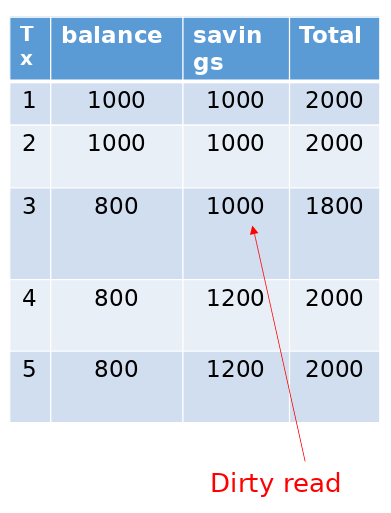
\includegraphics[width=0.25\textwidth]{dirty-reads.png}
    \caption{Dirty read example: every command Tx is a row}
\end{figure}

 

\textbf{Solutions:}

\begin{itemize}
    \item Read locks (=very bad performance)
    \item Remember the old value until commit
    \begin{itemize}
        \item Until the commit happens, every value will be what it was at Tx = 1
    \end{itemize}
\end{itemize}

\subsubsection{Dirty Writes}

\begin{theorem}[Dirty Write]
A dirty write happens when a transaction writes data that has been changed on disk by another transaction. 
The last transaction will overwrite what the first transaction wrote.
\end{theorem}


\begin{figure}[H]
    \centering
    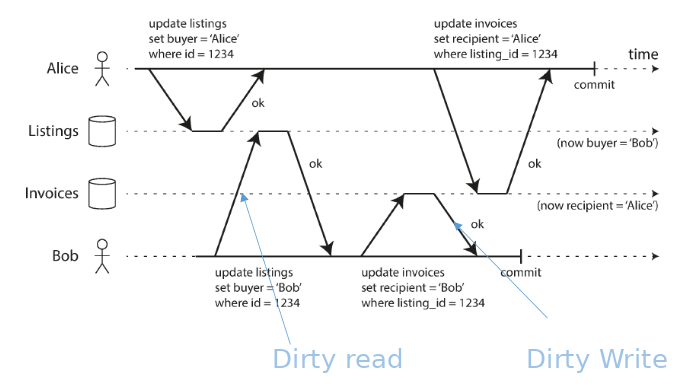
\includegraphics[width=0.6\textwidth]{dirty-reads-lock.png}
    \caption{Dirty write example}
\end{figure}

\begin{enumerate}
    \item Alice buys a car from a dealership
    \item Bob buys the same car from the dealership
    \item Bob gets an invoice before Alice because his internet is faster
    \item Alice gets an invoice after Bob. Two people now own the same car?
\end{enumerate}

\textbf{Solution: Write lock:}

\begin{itemize}
    \item If a row is claimed by a transaction, that row should be locked until commit
    \item Bob cannot write to the invoices, because it has been locked by Alice.
\end{itemize}

\subsubsection{Read skew}

\begin{theorem}[Read skew]
Read skew happens when a commit reads the same data twice, 
with different results because another transaction updated the data.
\end{theorem}

\begin{enumerate}
    \item Alice checks the balance of the first account
    \item Bob updates the balance of the first account
    \item Bob updates the balance of the second account
    \item Alice checks the balance of the second account
\end{enumerate}

Result: Alice `loses' \$100 in one commit, because another transaction changed data.

\begin{figure}[H]
    \centering
    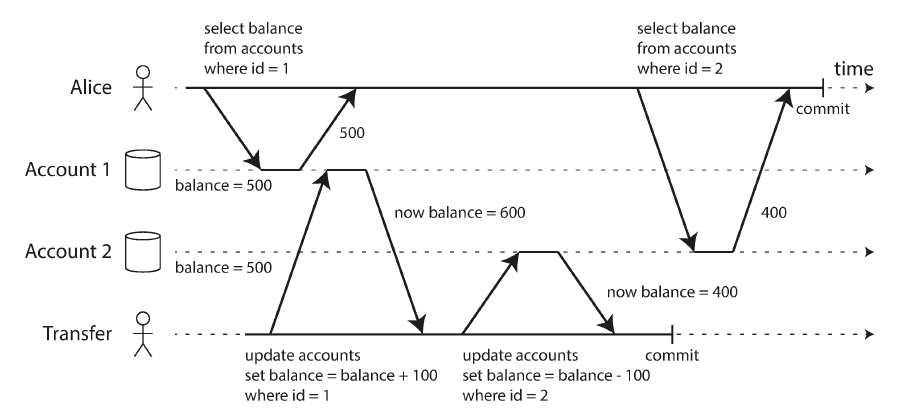
\includegraphics[width=0.6\textwidth]{read-skew.png}
    \caption{Read skew example}
\end{figure}

\textbf{Solution:}

\begin{itemize}
    \item Reading the values again solves the problem
    \item Except for backups: If a backup saves data while another transaction changes it, you will come across problems.
\end{itemize}


\subsubsection{Lost updates \& Atomic updates}

\begin{figure}[H]
    \centering
    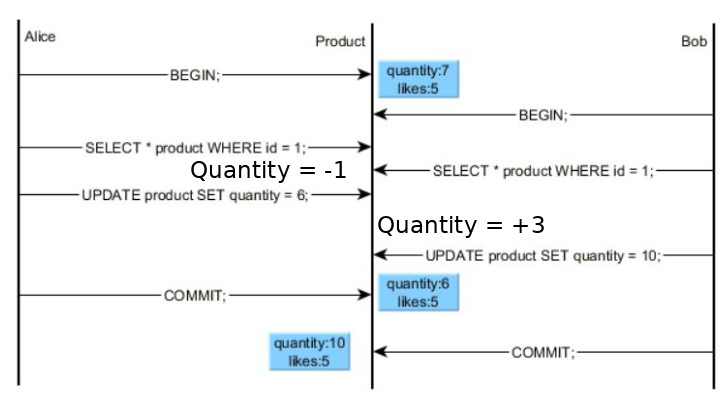
\includegraphics[width=0.5\textwidth]{lost-updates-atomic-updates.png}
    \caption{Lost updates: example}
\end{figure}

\begin{enumerate}
    \item Alice checks the quantity of the product (quantity = 7)
    \item Bob checks the quantity of the product (quantity = 7)
    \item Alice buys the product (quantity = 6)
    \item Bob thinks the quantity is 7 and he wants to add 3: he sets the quantity to 10 (7+3)
    \item Alice commits her changes. According to her, the quantity should be 6
    \item Bob commits his changes. The quantity is 10, overwriting Alice's changes. The actual quantity should be 9 (7-1+3)
\end{enumerate}

\textbf{Solution: Atomic updates}

\begin{itemize}
    \item Problem: Two read - modify - write transactions with different outcomes
    \item Repeatable read does not fix this
    \item Solutions: `atomic updates' or manual lock
    \begin{itemize}
        \item = Exclusive read lock on the data
        \item = No reads or update object until commit
        \item Update `X' SET value = "X2" $\Rightarrow$ (Read - modify - write in one operation)
    \end{itemize}
\end{itemize}

\subsubsection{Write Skew}

Atomic Updates don't protect against everything:

\begin{itemize}
    \item Multi object updates \& lost updates
\end{itemize}

Pattern:

\begin{enumerate}
    \item Read something
    \item Make decision
    \item Write new data
    \item By the time the write is committed, the premise of the decision (step 2) is no longer true.
\end{enumerate}

\subsubsection{2-phase lock - Serial execution}

With weak isolation levels:

\begin{itemize}
    \item Readers never block writers
    \item Writers never block readers (you can read the old value while it is being overwritten)
\end{itemize}

With 2-phase lock, there are two fases (duh):

\begin{enumerate}
    \item Exclusive read-lock on data
    \item Exclusive write-lock on data
\end{enumerate}

Problem: Deadlocks

\begin{itemize}
    \item Transactions keep waiting on other transactions' locks
    \item Result: the whole database can crash because of this
\end{itemize}

Examples that support 2-phase locking:

\begin{itemize}
    \item MySQL InnoDB
    \item SQL server
    \item DB2 (but DB2 mistakenly calls this "Repeatable read")
\end{itemize}

\subsection{Isolation levels}

= Choose between strong isolation or strong performance

\begin{itemize}
    \item Modern processing 8 - 100+ threads
    \item Choose an isolation level:
    \begin{itemize}
        \item Read Uncommitted (weakest isolation, most performance)
        \item Read Committed
        \item Repeatable Read (=snapshot isolation)
        \item Serial Execution (strongest isolation, least performance)
    \end{itemize}
    \item Isolation problems are hard to debug:
    \begin{itemize}
        \item It's a timing problem
        \item Very hard to reproduce
        \item No errors are logged
    \end{itemize}
\end{itemize}

\begin{figure}[H]
    \centering
    \includegraphics[width=0.7\textwidth]{isolation-levels-dbs.png}
    \caption{(default) isolation levels in current databases. (*) Wrong, Oracle does not comply with ANSI}
\end{figure}


\subsubsection{Isolation level 1: Read Uncommited}

\begin{itemize}
    \item Read Uncommitted offers no protection against concurrency threats
    \item Fastest performance, lowest isolation
    \item One transaction may see not-yet-committed changes made by other transactions
\end{itemize}


\subsubsection{Isolation level 2: Read Committed}

Offers protection against:

\begin{itemize}
    \item Dirty reads
    \item Dirty writes
\end{itemize}

\textbf{Solutions}

\begin{enumerate}
    \item Read locks (bad performance)
    \item Remember the old value until `commit' (better performance)
\end{enumerate}

\subsubsection{Isolation level 3: Repeatable read or Snapshot Isolation}

\begin{itemize}
    \item Also called "Multi Version Concurrency Control (MVCC)"
    \item Solves dirty reads, dirty writes and read skew
    \item If a commit happens before everything is fully backed up, every commit started after the start of the backup will be ignored.
    \item To accomplish this, every transaction gets a number
    \item `Readers do not block writes, writers do not block reads'
\end{itemize}


\subsubsection{Isolation level 4: Serial execution }

\begin{itemize}
    \item One single fast thread (in RAM) for writing
    \item Multiple threads for reading
    \item Not very fast, definitely not very scalable
    \item Only use if your database is not too complex
    \begin{itemize}
        \item Redis
        \item VoltDB
        \item Other databases that can be kept in memory\dots
    \end{itemize}
    \item No write locks necessary, no overhead from thread synchronisation, \dots
    \item Limited by a single thread on your CPU
    \item How to use multiple threads?
    \begin{itemize}
        \item Partition data
        \item Multiple threads, one thread per partition
        \item Speed will be much slower if a transaction accesses multiple partitions
    \end{itemize}
    \item Complete transaction in one serial stored procedure (=piece of code, already compiled and ready to execute)
\end{itemize}

\subsubsection{Conclusion}

\begin{itemize}
    \item Isolation levels are a complex trade-off between\dots:
    \begin{itemize}
        \item Consistency
        \item Scalability
    \end{itemize}
    \item Check your application: which level is the best for your usecase?
    \item 
\end{itemize}


\subsection{ACID: Durable}

= A database should be durable: every write transaction has to be written to disk, and should be stored safely and reliably.

But durability is also a trade-off: 

\begin{itemize}
    \item Higher durability $\Leftrightarrow$ lower performance
    \item Higher performance $\Rightarrow$ more risks
\end{itemize}


\subsubsection{Caching \& BBU}


\begin{itemize}
    \item If we choose the highest isolation on sofware, the hardware can still fail.
    \item For a RAID configuration:
    \begin{itemize}
        \item Most RAID configurations use a RAM cache before writing changes to disks
        \item RAM cache should have a Battery Backup Unit (BBU) in case the power goes out
        \item This is because RAM is by definition not durable, but volatile
    \end{itemize}
    \item Disks also have RAM caches
    \begin{itemize}
        \item This is mostly to sort the data before it gets written
        \item Use professional storage: disks with capacitors!
        \item RAM caches in SSDs have to be Non-Volatile (NV)!
    \end{itemize}
\end{itemize}

\subsubsection{The Transaction chain}

\begin{figure}[H]
    \centering
    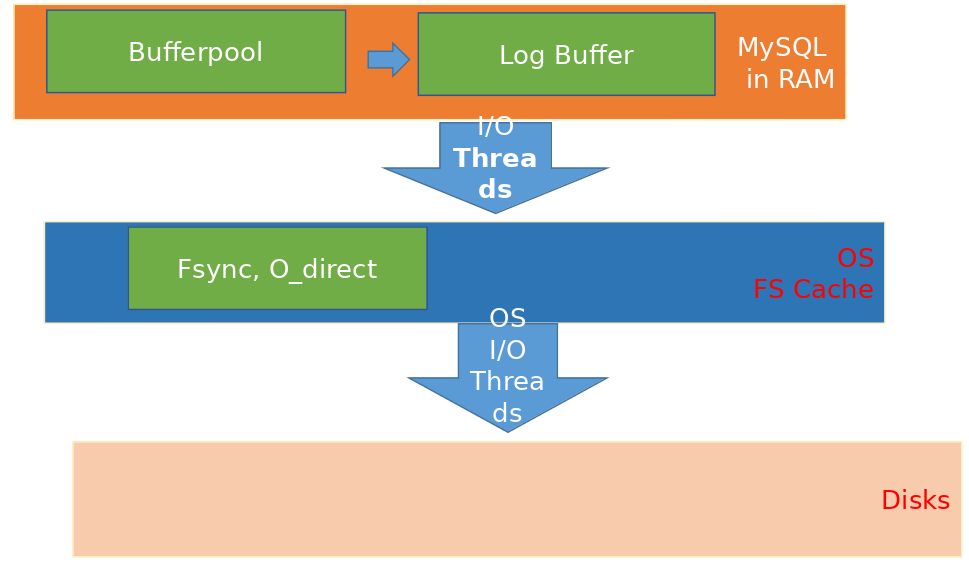
\includegraphics[width=0.5\textwidth]{transaction-chain.png}
    \caption{The transaction chain when writing to disk}
\end{figure}

Steps a transaction takes to write to disk:

\begin{enumerate}
    \item The transaction gets buffered in the buffer pool
    \item The data gets written to the log buffer
    \item Using multiple I/O threads, the log buffer gets flushed to the OS
    \item The OS chooses how the data is written (cache first, or write immediately)
    \item The OS writes the data to the disks
\end{enumerate}

\subsubsection{The transaction chain: innodb\_flush\_log\_at\_trx\_commit}

= a setting in MySQL InnoDB with three options:

\begin{itemize}
    \item 0: Write the log buffer to the log file and flush the log file \textbf{every second}, but do nothing at transaction commits (fastest)
    \begin{itemize}
        \item Fastest
    \end{itemize}
    \item 1: Write the log buffer to the log file and flush it to durable storage \textbf{at transaction commits}
    \begin{itemize}
        \item This is the only option that is fully ACID compliant
        \item It is also the slowest
    \end{itemize}
    \item 2: Write the log buffer to the log file \textbf{at every commit}, but flush it every second
\end{itemize}

\subsubsection{innodb\_flush\_method}

= a setting that tells the OS how the data has to be written

\begin{itemize}
    \item fdatasync
    \begin{itemize}
        \item InnoDB uses fsync() to flush both data and log files (unix)
    \end{itemize}
    \item O\_DIRECT
    \begin{itemize}
        \item This setting still uses fsync() to flush the files to disk, but it instructs the operating system not to cache the data and not to use read-ahead. Avoids double buffering
    \end{itemize}
    \item async\_unbuffered
    \begin{itemize}
        \item Default value on Windows
        \item Causes InnoDB to use unbuffered I/O for most writes
        \item Exception: it uses buffered I/O to the log files when innodb\_flush\_log\_at\_try\_commit = 2
    \end{itemize}
\end{itemize}

\begin{figure}[H]
    \centering
    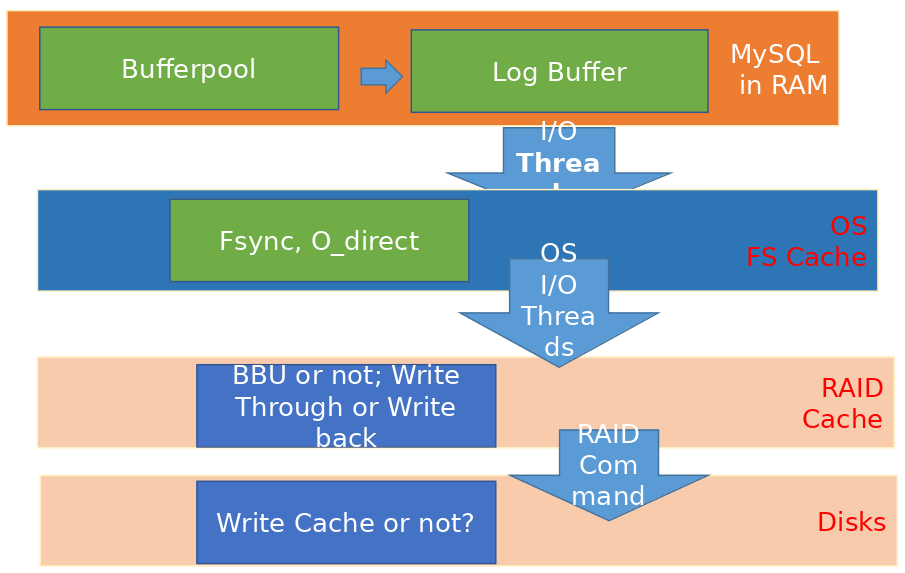
\includegraphics[width=0.5\textwidth]{transaction-chain2.png}
    \caption{The full transaction chain, with RAID}
\end{figure}

\section{NoSQL}

\subsection{SQL}

\subsubsection{Possibilities:}

\begin{itemize}
    \item Relationeel
    \item Column store 
    \item Document store
    \item Graph
    \item Key-value
    \item Specialisten:
    \begin{itemize}
        \item Time series
        \item Text search
    \end{itemize}
\end{itemize}

\begin{figure}[H]
    \centering
    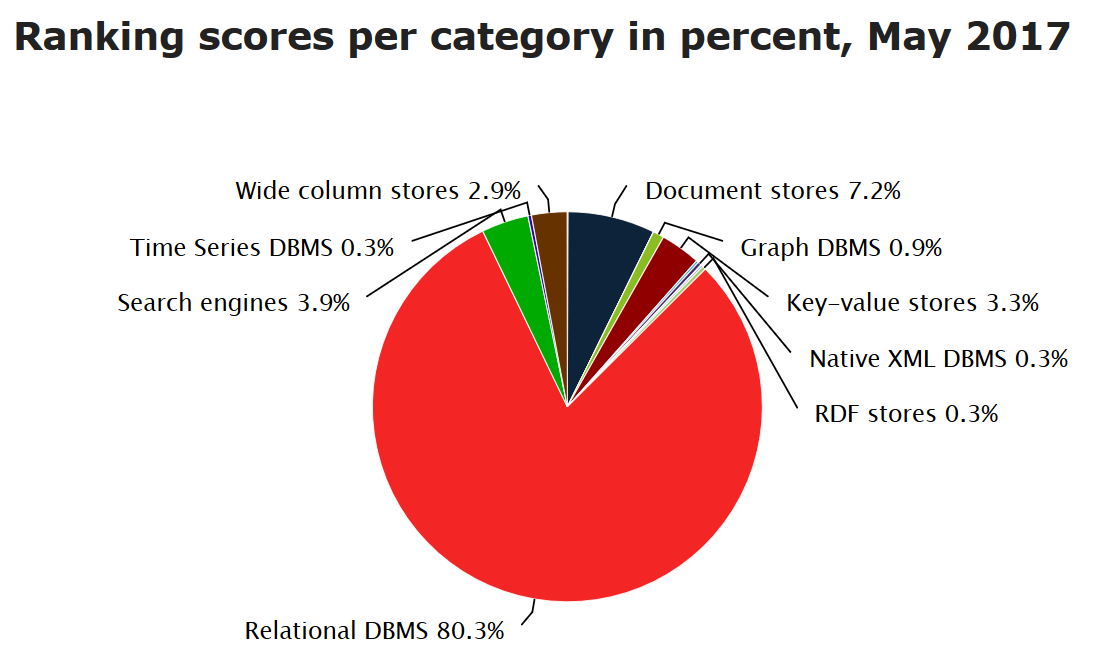
\includegraphics[width=0.5\textwidth]{sql-piechart.png}
    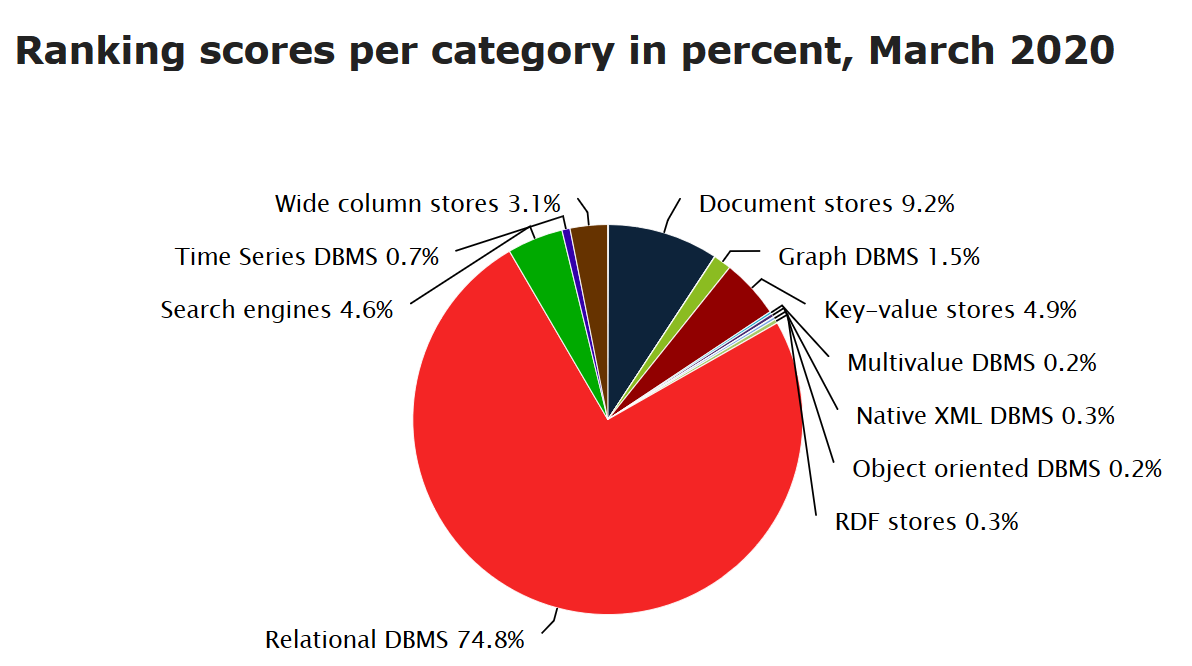
\includegraphics[width=0.5\textwidth]{sql-piechart2.png}
    \caption{Popularity: Relational DBs are the most popular}
\end{figure}

\subsubsection{Imperative languages vs Declarative languages}

\begin{figure}[H]
    \centering
    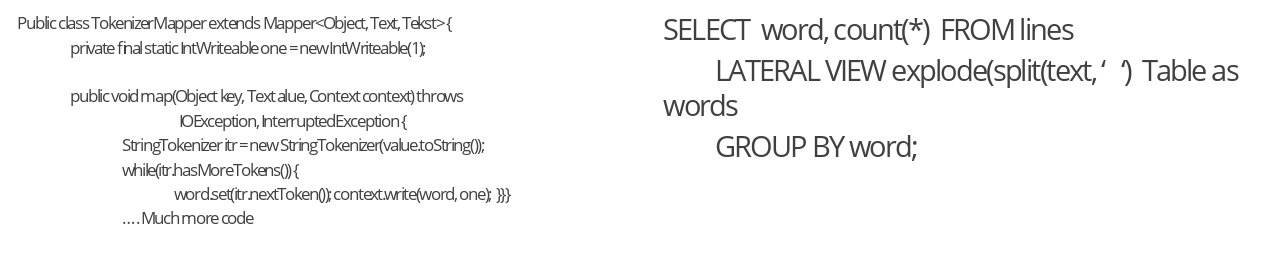
\includegraphics[width=0.7\textwidth]{imperative-vs-declarative.png}
    \caption{Imperative (left) vs Declarative languages (right)}
\end{figure}

\begin{itemize}
    \item Imperative: tell the system how to retrieve/handle/mutate the data, in what order
    \begin{itemize}
        \item C\#, python, \dots
    \end{itemize}
    \item Tell the system the structure of the data you're looking for. Don't tell the system how it has to happen, the query optimizer.
    \begin{itemize}
        \item SQL, HTML + CSS
    \end{itemize}
\end{itemize}

\subsection{Index}

Index of a book:

\begin{itemize}
    \item Summary/copy that allows to search faster in the main structure (book/database)
    \item Redundant (copy), needs disk space (needs "pages")
\end{itemize}

Index of a database:

\begin{theorem}[Index]
    A copy of some columns from a table, sorted, that improves the speed of data retrievel operations at the cost of additional writes and storage space to 

    TODO
\end{theorem}

\url{https://use-the-index-luke.com/sql/anatomy}

\subsubsection{B-tree index}

\begin{figure}[H]
    \centering
    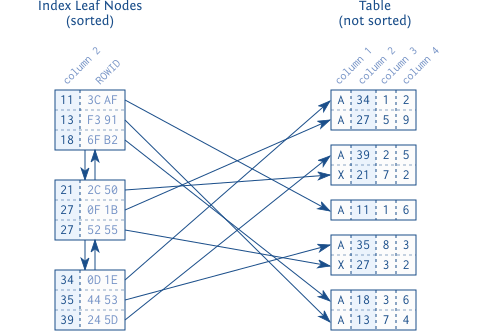
\includegraphics[width=0.5\textwidth]{b-tree-index.png}
    \caption{}
\end{figure}

\begin{itemize}
    \item Leaf nodes = a double linked list
    \begin{itemize}
        \item Index + Row ID
        \item or index + value (in `key value' DBs)
        \item Every block refers to other blocks: the next and previous block
        \item insert = add new links to the list
    \end{itemize}
    \item This index is stored in RAM:
    \begin{itemize}
        \item every block refers to another block
        \item If you have to jump to another block, sequential disks are too slow for random access
        \item random read/writes are much faster with RAM
        \item If you have 10 million records: serial search is way too slow!
    \end{itemize}
\end{itemize}

\subsubsection{Tree architecture}

\begin{figure}[H]
    \centering
    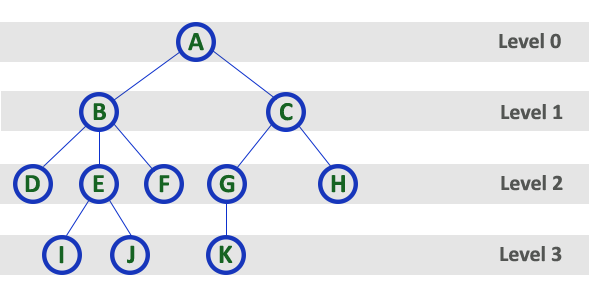
\includegraphics[width=0.5\textwidth]{tree-architecture.png}
    \caption{A balanced tree}
\end{figure}

\begin{itemize}
    \item A = root
    \item B \& C = child (pages)
    \item AC = edge
    \item Depth A to K = 3 (=amount of edges)
    \begin{itemize}
        \item From root to leaf
    \end{itemize}
    \item I, J, K = leaf nodes (point to data)
\end{itemize}

\subsubsection{Searching for an index}

\begin{figure}[H]
    \centering
    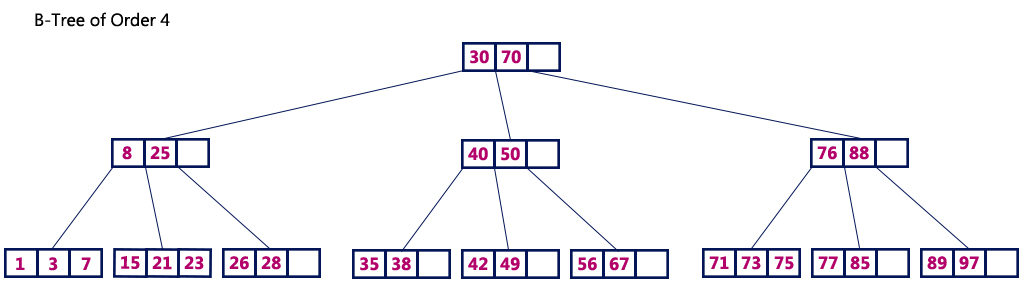
\includegraphics[width=0.5\textwidth]{balanced-tree-index.png}
    \caption{Balanced tree example}
\end{figure}

Find 38:

\begin{enumerate}
    \item Search from node 30
    \item Find subnode 40
    \item Search from node 35 (depth 3), now read serially
    \item Find row id in index 38
\end{enumerate}

\subsubsection{Size}

\begin{itemize}
    \item Block size = 16KB
    \item Branching factor = 100 (=amount of nodes in a page)
    \item Depth = 3
    \item $100 \cdot 100 \cdot 100 \cdot 16\text{KB} = 16\text{GB}$
    \begin{itemize}
        \item Typical depth: 4
        \item Typical branches = 100s
    \end{itemize}
\end{itemize}

\subsubsection{B-trees: getting faster \& more reliable}

\begin{itemize}
    \item WAL (Write Ahead Log) or REDO log = sequential database
    \begin{itemize}
        \item append only
        \item update are critical moments
    \end{itemize}
    \item 1 update = two writes
    \begin{itemize}
        \item WAL
        \item Page update
    \end{itemize}
    \item Less levels vs more branches:
    \begin{itemize}
        \item Each level can be a disk seek
        \item Using  means less disk seeks
    \end{itemize}
\end{itemize}

TODO

\subsubsection{Python + Postgres}

Python + Postgres can handle almost any analytics challenge

\begin{figure}[H]
    \centering
    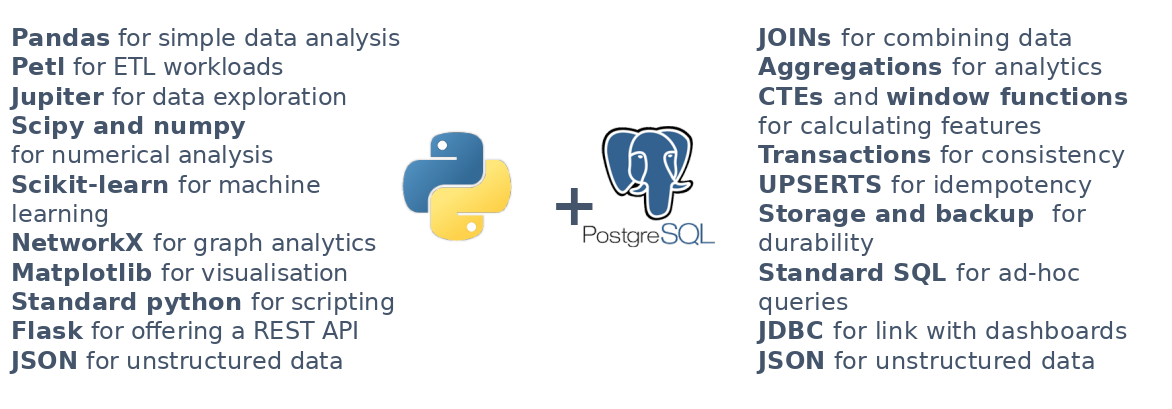
\includegraphics[width=0.5\textwidth]{python-postgres.png}
    \caption{}
\end{figure}

\subsubsection{When is SQL not the answer}

\begin{itemize}
    \item Volume = When you have petabytes of data (rare)
    \item Velocity = Too many writes per second
    \item Scalability
    \begin{itemize}
        \item Want to avoid expensive servers
        \item Want to avoid expensive SANs (Storage Area Network)
    \end{itemize}
    \item Variety = When you don't want to turn an object (with unstructured data) into a relational row
    \begin{itemize}
        \item = Object - relational database mismatch
        \item \url{https://en.wikipedia.org/wiki/Object%E2%80%93relational_impedance_mismatch}
    \end{itemize}
\end{itemize}

\subsection{Key-Value}

TODO: betere image

\begin{figure}[H]
    \centering
    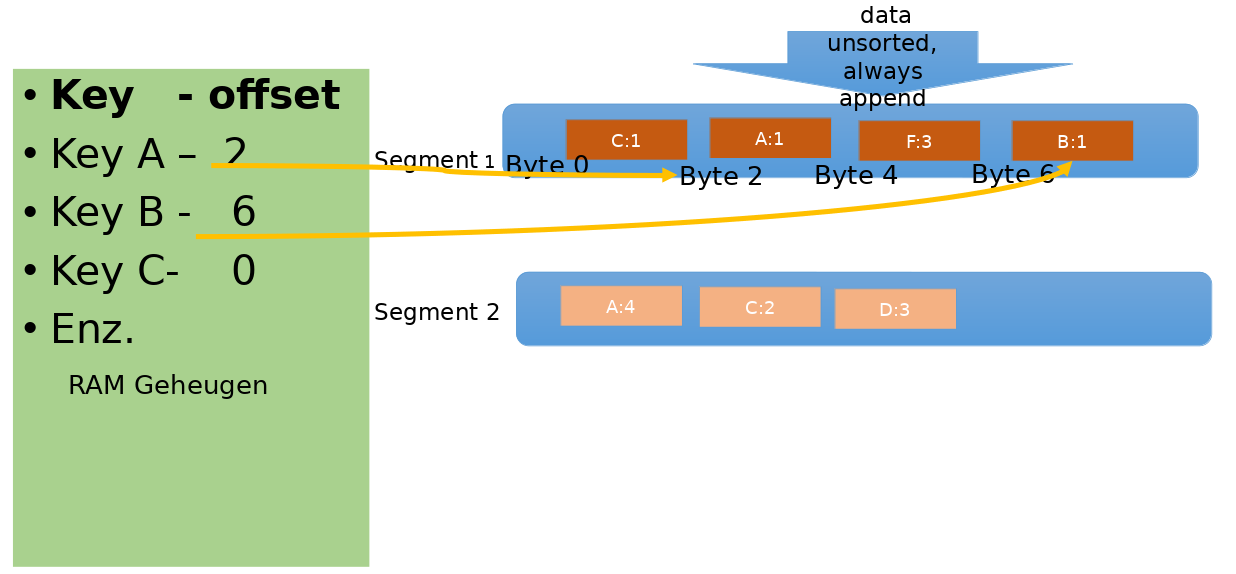
\includegraphics[width=0.5\textwidth]{key-value.png}
    \caption{Log structure + hash index}
\end{figure}

\begin{itemize}
    \item TODO
    \item 
\end{itemize}

\subsubsection{Compacting}

TODO: betere image

\begin{figure}[H]
    \centering
    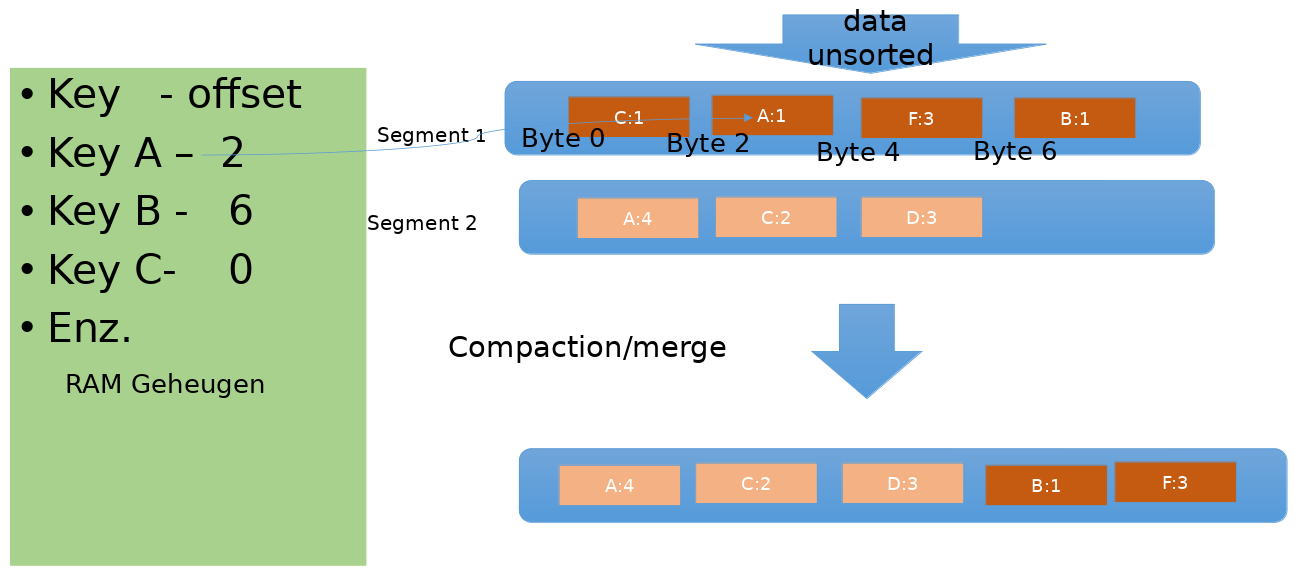
\includegraphics[width=0.5\textwidth]{key-value-compacting.png}
    \caption{Compaction/merge of 2 segments}
\end{figure}

\begin{itemize}
    \item TODO
    \item Segment 2 is newer: we ignore the first segment's A and B
\end{itemize}

\subsubsection{Principles}

\begin{itemize}
    \item Very fast writes (append only: you can write sequentially because disks don't need to change tracks)
    \item When crash: no corruption because of wrong update
    \item very fast reads if hash index is in RAM
    \begin{itemize}
        \item if not: very slow
        \item SELECT * FROM A TO ZZZ (ordered full scan == slooow)
    \end{itemize}
    \item Example Riak Bitcask (\url{https://en.wikipedia.org/wiki/Riak})
\end{itemize}

\subsection{LSM: Log Structured Merge Tree}

\begin{figure}[H]
    \centering
    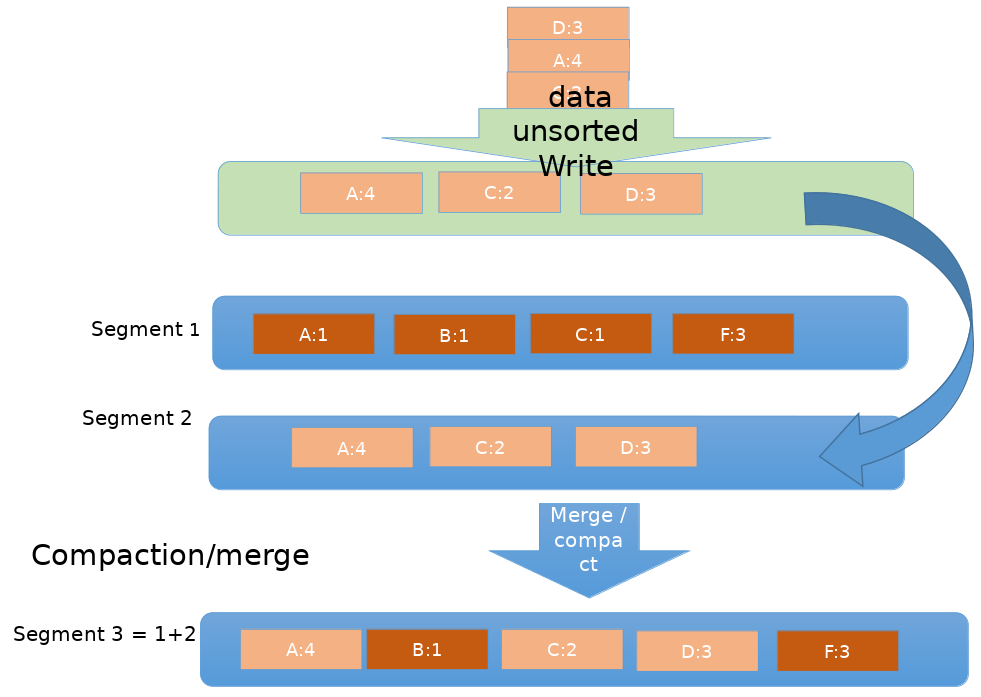
\includegraphics[width=0.5\textwidth]{lsm.png}
    \caption{}
\end{figure}

TODO: betere image

\begin{itemize}
    \item Sort in RAM (memtable)
    \begin{itemize}
        \item Log segment file as backup
    \end{itemize}
    \item Write to disk after several MB
    \begin{itemize}
        \item To sorted string table file
    \end{itemize}
    \item Merge, compact and sort
    \item TODO
\end{itemize}

\subsubsection{Log Structure Merge + Sparse tree index}

\begin{itemize}
    \item We can simplify the LSM
    \item Sparse tree index = remember where some milestones are
    \begin{itemize}
        \item If you need F, and you know where D and G are
        \item Start reading from D (byte-offset 10800)
        \item Read sequentially until G (byte-offset 11000)
        \item This sequential read is very quick, because 
    \end{itemize}
    \item Merge, compact \& sort every time = string sorted table
    \item Every delete: create new segment and merge. `Tombstone the old segment'
\end{itemize}

\subsubsection{Applications of Sorted String \& LSM-tree}

\begin{itemize}
    \item First application: Google Big Table (\url{https://en.wikipedia.org/wiki/Bigtable})
    \item LevelDB, Rocks-DB
    \item Hbase, Cassandra (Facebook)
    \item ElasticSearch: Lucene text search (key = text, value = document) or inverted index
\end{itemize}

\subsubsection{Advantages LSM}

\begin{itemize}
    \item Very fast writes
    \item Quite fast reads (sparse index)
    \item Easily scaled over nodes (segments)
\end{itemize}

\subsubsection{Disadvantages LSM}

\begin{itemize}
    \item Write (merge \& delete) in background can influence speeds
    \item Deletes are costly!
    \item You have to specify the rate between compaction \& write/read (ongoing action) yourself
\end{itemize}

\subsubsection{Summary: B-Trees vs LSM trees}

\begin{itemize}
    \item TODO
\end{itemize}

\subsection{Time Series}

= LSM with a twist

\begin{figure}[H]
    \centering
    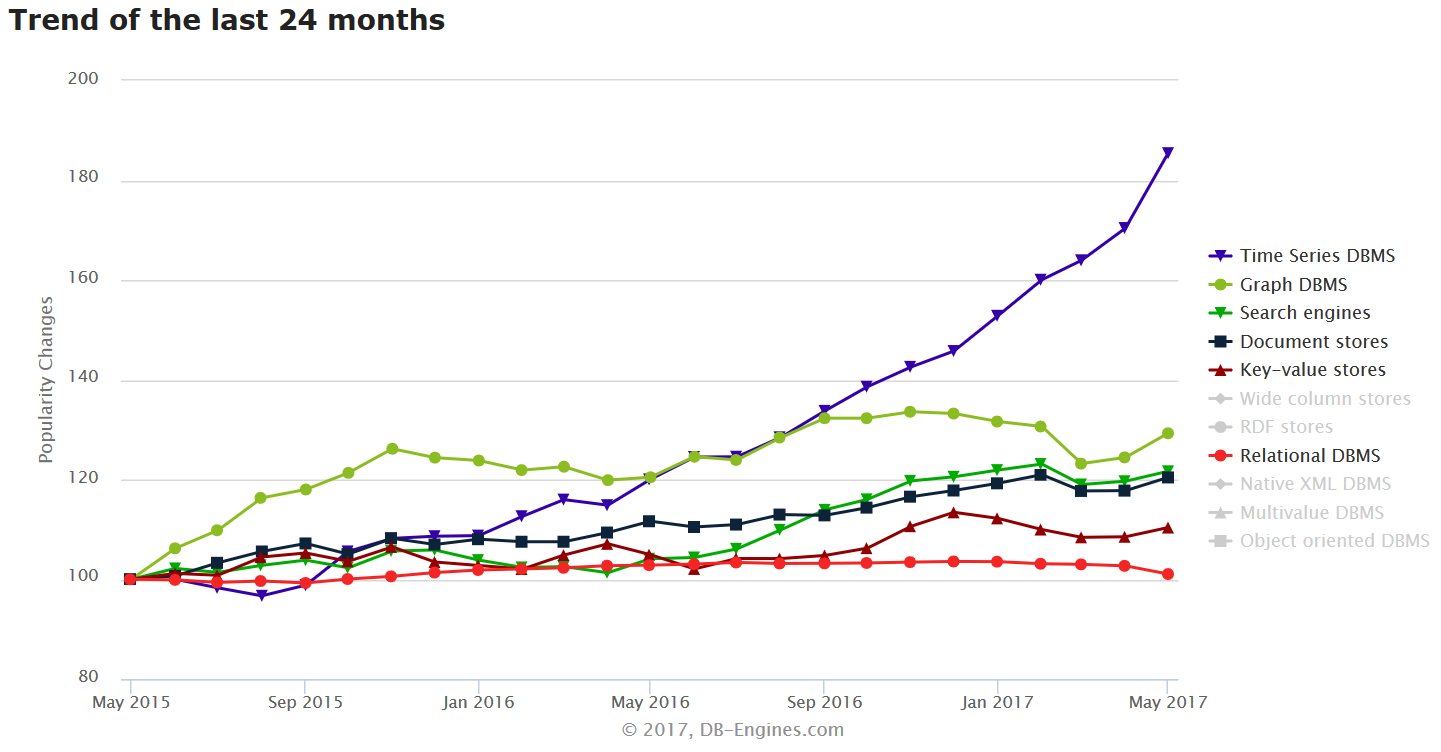
\includegraphics[width=0.5\textwidth]{time-series-lsm.png}
    \caption{Popularity}
\end{figure}

\subsubsection{Properties}

\begin{itemize}
    \item Lots of individual data points: `a row is not important'
    \item High write throughput
    \item High read throughput (aggregation per hour/day)
    \item Large deletes (data expiration)
    \item Mostly an insert/append workload, very few updates
\end{itemize}

\subsubsection{Use case: windmill sensors}

Situation: a windmill has many sensors that produce data that needs to be logged

\begin{itemize}
    \item Turbine sensor data needs to be stored every second
    \begin{itemize}
        \item 30 sensor readings per second
        \item > 300GB per windmill per year
    \end{itemize}
    \item Both aggreation as realtime
    \item Issue: MySQL database read locks during queries, INSERT failed, causing data loss
\end{itemize}

\subsubsection{Case study: influx DB}

\url{https://docs.influxdata.com/influxdb/v1.4/concepts/storage_engine/}

TODO: `read the entire page and understand everything, and answer these questions:'

\begin{itemize}
    \item Why important for MCT?
    \item How can you scale?
    \item TSM?
    \item WAL? How durable? What is it?
    \item What is a compactor? Compaction planning?
    \item Give one example of unique functionality typical for a time series environment
    \begin{itemize}
        \item Tip: say you need to aggregate every hour
    \end{itemize}
\end{itemize}

\subsection{Object - relational mismatch}

\begin{figure}[H]
    \centering
    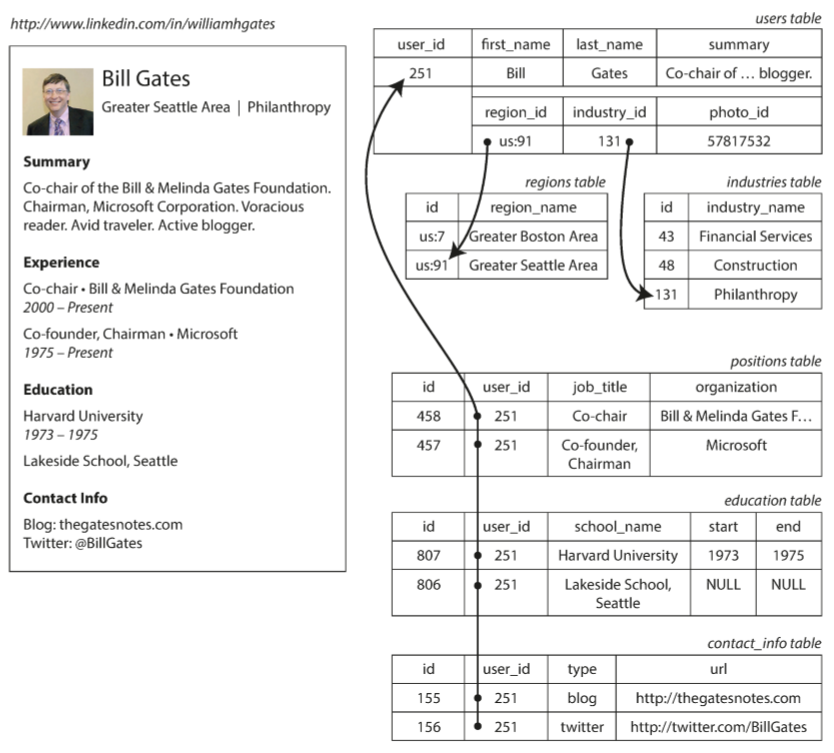
\includegraphics[width=0.5\textwidth]{billgates.png}
    \caption{Representing an object in relational rows}
\end{figure}

\begin{itemize}
    \item TODO
    \item Better match for objects with unstructured data: JSON documents
\end{itemize}

\subsubsection{PostgreSQL}

\begin{itemize}
    \item Mid 2014: PostgreSQL 9.4 natively supports JSON
    \item The speed to ingest documents as quickly as MongoDB, but ACID!
    \item Fully indexable
\end{itemize}

\subsection{ElasticSearch}

\begin{itemize}
    \item Document Store
    \begin{itemize}
        \item So naturally suited for describing objects
        \item JSON serialized
    \end{itemize}
    \item Easy access to an advanced fulltext search-engine library
    \item Lucene is very complex but very advanced
    \item Automatized sharding (and thus scalable) in containers
    \item RESTful API
    \item Slower data ingest (`index')
\end{itemize}

\subsubsection{Elastic Search architecture}

\begin{itemize}
    \item Document = JSON data
    \item Index = a collection of documents
    \item Shards = scalable pieces of index
    \item Segments = sequential pieces of a shard
\end{itemize}

\begin{figure}[H]
    \centering
    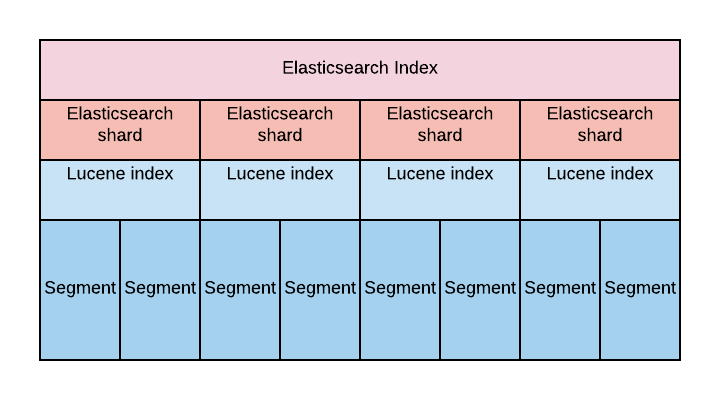
\includegraphics[width=0.5\textwidth]{elasticsearch-architecture.png}
    \caption{}
\end{figure}

\subsubsection{Elastic Search Cluster}

\begin{itemize}
    \item Index is split over shards - nodes: scalability
    \item Shards can be replicated over nodes: availability
\end{itemize}

\begin{figure}[H]
    \centering
    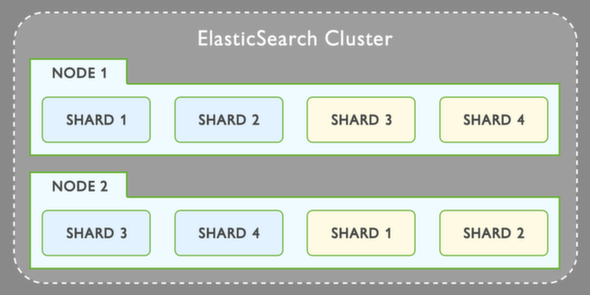
\includegraphics[width=0.5\textwidth]{elasticsearch-searchcluster.png}
    \caption{}
\end{figure}

\subsubsection{Inverted index}

\begin{itemize}
    \item TODO
    \item = `Lucene Index'
\end{itemize}

\subsubsection{GeoHashes: Representing Geospatial data in ElasticSearch}

\begin{itemize}
    \item Since ElasticSearch 0.90
    \item Base32 encoded strings, interleaving the latitude and longitude
    \item Max resolution: 40mm * 20mm
    \item Each extra symbol divides the grid in 26 cells
    \item Use ElasticSearch's text search capabilities
\end{itemize}

\begin{figure}[H]
    \centering
    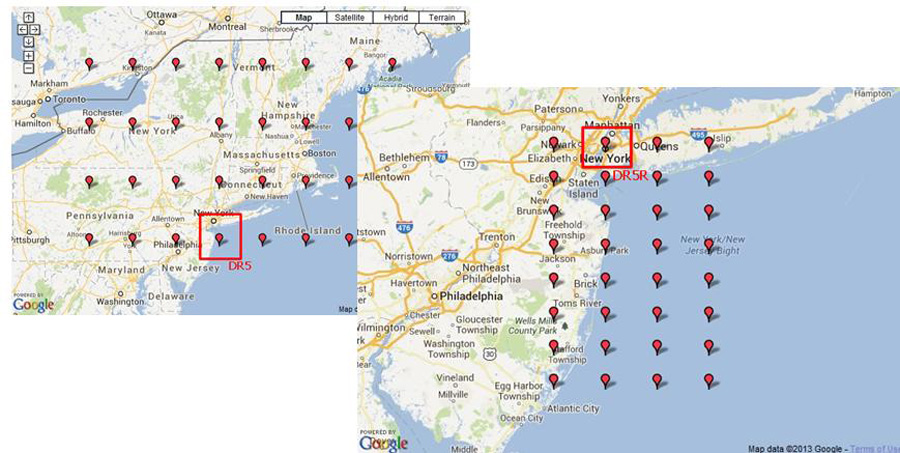
\includegraphics[width=0.5\textwidth]{geohashes.jpg}
    \caption{}
\end{figure}

\subsubsection{ElasticSearch scaling}

\begin{figure}[H]
    \centering
    \includegraphics[width=0.5\textwidth]{elasticsearch-scaling.png}
    \caption{}
\end{figure}

\subsection{Which storage engine is the best and the worst}

Which storage engine is the best/worst for the following situations:

\begin{itemize}
    \item High amount of writes every second (sensor data)
    \item Hoog aantal updates iedere seconde 
    \begin{itemize}
        \item Web analyse data (Marketing campagne)
    \end{itemize} 
    \item Constante updates en reads van persoonlijke data? 
    \item Full scans op gestructureerde data?
    \item ACID compliant OLTP?
\end{itemize}


\end{document}